\subsection{Model ISO/OSI}
Počítačové sítě vyvíjelo více firem, zpočátku to byly uzavřené a nekompatibilní systémy. Hlavním účelem sítí je však vzájemné propojování, a tak vyvstala potřeba stanovit pravidla pro přenos dat v sítích a mezi nimi. \textbf{Mezinárodní ústav pro normalizaci ISO} (International Standards Organization) vypracoval tzv. referenční model \textbf{OSI (Open Systems Interconnection)}, který rozdělil práci v síti do \textbf{7 vzájemně spolupracujících vrstev}.

Princip spočívá v tom, že vyšší vrstva převezme úkol od podřízené vrstvy, zpracuje jej a předá vrstvě nadřízené. Vertikální spolupráce mezi vrstvami (nadřízená s podřízenou) je \textbf{věcí výrobce} sítě. Model \textbf{ISO/OSI doporučuje}, jak mají vrstvy \textbf{spolupracovat horizontálně} – dvě stejné vrstvy modelu mezi různými sítěmi (či síťové prvky různých výrobců). Model je důležitý především pro výrobce síťových komponent. V praktické práci se sítí jej moc nevyužijeme. Umožňuje však pochopit principy práce síťových prvků a zároveň patří k základní terminologii sítí.

\begin{itemize}
\item\textbf{Aplikační vrstva }- je \textbf{určitou aplikací} (např. oknem v programu) zpřístupňující uživatelům síťové služby. Nabízí a zajišťuje přístup k souborům (na jiných počítačích), vzdálený přístup k tiskárnám, správu sítě, elektronické zprávy (včetně e-mailu).
\item\textbf{Prezentační vrstva} - má na starosti \textbf{konverzi dat}, přenášená data mohou totiž být v různých sítích různě kódována. Tato vrstva zajišťuje sjednocení formy vzájemně přenášených údajů. Dále data komprimuje, případně šifruje. V praxi často splývá s relační vrstvou.
\item \textbf{Relační vrstva} - \textbf{navazuje} a po skončení přenosu \textbf{ukončuje} \textbf{spojení}. Může provádět \textbf{ověřování} uživatelů, \textbf{zabezpečení} přístupu k zařízením.
\item\textbf{Transportní vrstva} - vrstva\textbf{ zajišťuje přenos dat mezi koncovými uzly}. Jejím účelem je poskytnout takovou kvalitu přenosu, jakou požadují vyšší vrstvy. Vrstva nabízí spojově (TCP) a nespojově orientované (UDP) protokoly. (Platí pouze pro \textbf{TCP/IP})
\item\textbf{Síťová vrstva }- je zodpovědná za spojení a \textbf{směrování mezi dvěma počítači nebo celými sítěmi} (tj. uzly), mezi nimiž neexistuje přímé spojení. Stará se o síťové adresování.
\item \textbf{Linková (spojová) vrstva }- poskytuje \textbf{spojení mezi dvěma sousedními systémy}. \textbf{Uspořádává data} z fyzické vrstvy do logických celků známých jako \textbf{rámce} (frames). Seřazuje přenášené rámce, stará se o nastavení parametrů přenosu linky, oznamuje neopravitelné chyby. Formátuje fyzické rámce, opatřuje je fyzickou adresou a poskytuje synchronizaci pro fyzickou vrstvu.
\item\textbf{Fyzická vrstva }- fyzická vrstva definuje všechny elektrické a fyzikální vlastnosti zařízení. Jakým signálem je reprezentována logická jednička, jak přijímací stanice rozezná začátek bitu, jaký je tvar konektoru, k čemu je který vodič v kabelu použit.
\end{itemize}

\subsection{TCP/IP}
Rodina protokolů TCP/IP (Transmission Control Protocol/Internet Protocol) obsahuje \textbf{sadu protokolů} pro komunikaci v počítačové síti a je hlavním protokolem celosvětové sítě \textbf{Internet}. 

\textbf{Komunikační protokol} je množina pravidel, která určují syntaxi a význam jednotlivých zpráv při komunikaci. Architektura TCP/IP je členěna do čtyř vrstev (na rozdíl od referenčního modelu OSI se sedmi vrstvami):

\begin{enumerate}
	\item \textbf{Vrstva síťového rozhraní} (Network interface)
	\item \textbf{Síťová (IP) vrstva} (Internet layer)
	\item \textbf{Transportní vrstva} (Transport layer)
	\item \textbf{Aplikační vrstva }(Application layer)
\end{enumerate}

\noindent\makebox[\textwidth]{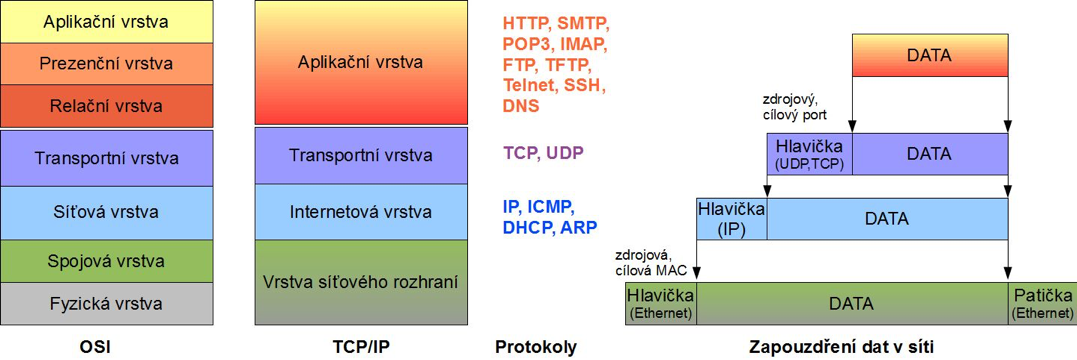
\includegraphics[width=\textwidth]{assets/4_tcpip}}

Komunikace mezi \textbf{stejnými vrstvami dvou různých systémů} je řízena \textbf{komunikačním protokolem} za použití spojení vytvořeného sousední nižší vrstvou. Architektura umožňuje výměnu protokolů jedné vrstvy bez dopadu na ostatní. Příkladem může být možnost komunikace po různých médiích fyzické vrstvy modelu OSI - ethernet (optické vlákno, kroucená dvojlinka, Wi-Fi), sériová linka.


\subsection{Vrstva síťového rozhraní}
Nejnižší vrstva umožňuje \textbf{přístup k fyzickému přenosovému médiu}. Je specifická pro každou síť v závislosti na její implementaci. Příklady sítí: 
\begin{itemize}
\item \textbf{Ethernet} --  název souhrnu technologií pro počítačové sítě (LAN, MAN) z větší části standardizovaných jako \textbf{IEEE 802.3}, které používají kabely s \textbf{kroucenou dvoulinkou}, optické kabely (ve starší verzích i koaxiální kabely) pro komunikaci přenosovými rychlostmi od 1 Mbit/s po 100 Gbit/s.
\item \textbf{Token ring} -- technologie lokální sítě. Principem je předávání vysílacího práva pomocí speciálního rámce (tzv. tokenu) mezi adaptéry, zapojenými do logického kruhu.
\item \textbf{FDDI} -- síť kruhovou topologií (dva kruhy pro opačné směry přenosu), používá optické kabely.
\item \textbf{X.25} (později nahrazena Frame Relay), \textbf{SMDS}.
\end{itemize}


\subsection{Síťová vrstva}
Vrstva zajišťuje \textbf{především síťovou adresaci}, \textbf{směrování} a předávání datagramů (\textbf{packety}). Je implementována ve všech prvcích sítě - \textbf{směrovačích} i \textbf{koncových zařízeních}. Protokoly:
\begin{itemize}
\item \textbf{IP (Internet Protokol)} -- základní protokol pro přenos dat po sítí. Sám nezaručuje nic. Podle IP adres jen směruje paket k cíli.
\item \textbf{ICMP (Internet Control Message Protocol)} -- slouží pro odesílání chybových zpráv např. že služba není dostupná.
\item \textbf{ARP (Adress Resolution Protocol)} -- převádí IP adresy na MAC adresy
\item \textbf{DHCP (Dynamic Host Configuration Protocol)} -- požívá se pro automatickou konfiguraci počítačů připojených do sítě. Přiděluje například IP adresy.
\end{itemize}

\subsubsection{Protokol IP (Internet Protocol)}
Od nadřazených protokolů transportní vrstvy obdrží datové segmenty s požadavkem na odeslání. K segmentům připojí vlastní hlavičku a vytvoří IP datagram. V IP hlavičce je především IP adresa příjemce a odesílatele. IP protokol je \textbf{nespojový} (před zahájením výměny dat nevytváří relaci) a \textbf{nespolehlivý} (předání paketů na místo určení není kontrolováno). Paket IP se tedy může ztratit, být doručen mimo pořadí, zdvojen nebo zpožděn. Protokol IP neobsahuje prostředky pro zotavení z chyb tohoto typu. To vše má zajistit nadřízená transportní vrstva – protokol \textbf{TCP}.

\subsection{Transportní vrstva}
Transportní vrstva je implementována až v \textbf{koncových zařízeních} (počítačích), a umožňuje proto přizpůsobit chování sítě potřebám aplikace. Poskytuje transportní služby kontrolovaným spojením \textbf{spolehlivým} protokolem \textbf{TCP} (transmission control protocol) nebo nekontrolovaným spojením \textbf{nespolehlivým} protokolem \textbf{UDP} (user datagram protocol).

\subsubsection{TCP (Transmission Control Protocol)}
Vytváří \textbf{virtuální okruh} mezi koncovými aplikacemi a zajišťuje tedy spolehlivý přenos dat.
\begin{itemize}
	\item Spolehlivá transportní služba, doručí adresátovi všechna data \textbf{bez ztráty} a ve \textbf{správném pořadí}.
	\item Služba se spojením, má fáze \textbf{navázání spojení} (3-way handshake), \textbf{přenos dat} a \textbf{ukončení spojení}.
	\item Transparentní přenos libovolných dat.
	\item \textbf{Plně duplexní spojení}, současný obousměrný přenos dat.
	\item Rozlišování aplikací pomocí portů.
	\item Komunikace je řízená pomocí \textbf{příznakových bitů} (ACK, SYN, atd.)
\end{itemize}

\begin{figure}[H]
	\centering
	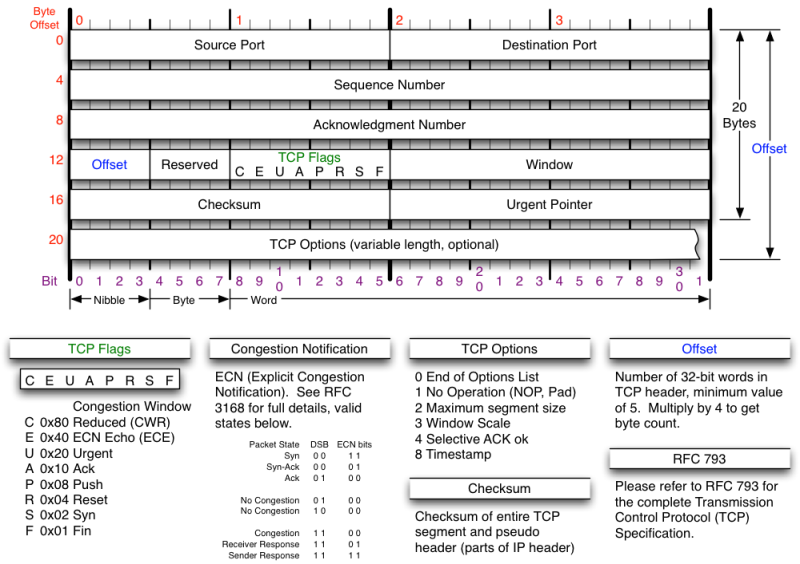
\includegraphics[width=\textwidth]{assets/4_tcp}
\end{figure}

\subsubsection{UDP (User Datagram Protocol)}
Poskytuje \textbf{nespolehlivou} transportní službu pro takové aplikace, které nepotřebují spolehlivost, jakou má protokol TCP a jde jim čistě o \textbf{rychlost}. Nemá fázi navazování a ukončení spojení a už první segment UDP obsahuje aplikační data. UDP je používán aplikacemi jako je \textbf{DHCP}, \textbf{TFTP}, \textbf{SNMP}, \textbf{DNS} a \textbf{BOOTP}.
\begin{itemize}
	\item Nespolehlivá transportní služba, \textbf{neověřuje} zda data došla v pořádku nebo ve správném pořadí.
	\item Nižší režie než u TCP (\textbf{rychlejší}).
	\item Zajištění spolehlivosti je na aplikacích vyšší vrstvy.
	\item Nemá fázi navázání a ukončení spojení, rovnou zasílá data.
	\item Hlavička UDP má pouze 4 části (délku, zdrojový/cílový port, checksum)
\end{itemize}

\noindent\makebox[\textwidth]{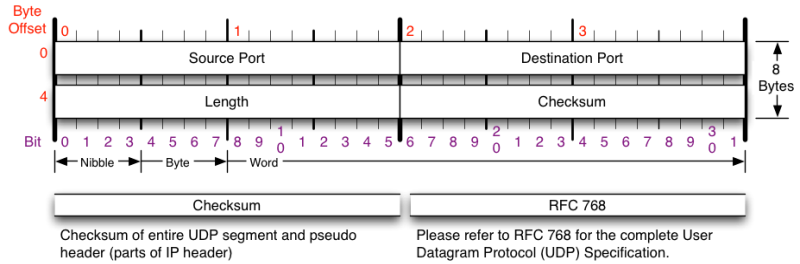
\includegraphics[width=14cm]{assets/4_udp}}

\subsection{Aplikační vrstva}
Jedná se přímo o programy (procesy), které využívají přenosu dat po síti ke konkrétním službám pro uživatele. Příklady: \textbf{Telnet} (TCP 23), \textbf{FTP} (TCP 20, 21), \textbf{HTTP} (TCP 80), \textbf{DHCP} (TCP/UDP 67, 68), \textbf{DNS} (TCP/UDP 53), \textbf{SSH} (TCP 22), \textbf{SMTP} (TCP/UDP 25), \textbf{POP3} (TCP 110), \textbf{IMAP} (TCP 143).

Aplikační protokoly používají vždy jednu ze dvou základních služeb transportní vrstvy: \textbf{TCP} nebo \textbf{UDP}, případně obě dvě (např. DNS). Pro rozlišení aplikačních protokolů se používají tzv. \textbf{porty}, což jsou domluvená číselná označení aplikací. Každé síťové spojení aplikace je jednoznačně určeno \textbf{číslem portu} a \textbf{transportním protokolem} (a samozřejmě adresou počítače).